\documentclass[a4paper]{ltjsarticle}
\usepackage{graphicx}
\usepackage{enumitem}
\usepackage{siunitx}
\usepackage{multirow}
\usepackage{cprotect}

\setlist[enumerate,1]{label= \textcircled{\scriptsize \arabic*}}
\setlist[enumerate,2]{label= \arabic*.}

%% Hyphenation setting
\hyphenpenalty=1000\relax
\exhyphenpenalty=1000\relax
\sloppy

\makeatletter

\def\Hline{
    \noalign{\ifnum0=`}\fi\hrule \@height 3.\arrayrulewidth \futurelet
    \reserved@a\@xhline}
\makeatother

\begin{document}
% ------------------------------------------------------
% front cover
% ------------------------------------------------------

\large
\vspace{-5.0cm}
\hspace{-1.0cm}
情報工学実験II

\hspace{-1.0cm}
2019年5月8日

\Huge
\vspace{1.0cm}
\begin{center}
    食堂システム 外部・内部設計書
\end{center}

\vspace{0.5cm}
\begin{center}
    \LARGE
    明石工業高等専門学校
\end{center}

\LARGE
\begin{center}
    \begin{tabular}{rl}
        E1507 & 泉 和哉 \\
        E1514 & 岡本 一真 \\
        E1533 & 西 総一朗
    \end{tabular}
\end{center}

\normalsize

\tableofcontents
\thispagestyle{empty}
\clearpage
\setcounter{page}{1}

% ------------------------------------------------------
% text start
% ------------------------------------------------------

\section{外部設計}
\subsection{システム}
    \subsubsection{サーバー構成}
        表\ref{tab:server_hardware},\,\ref{tab:server_software}にサーバーの構成を示す.
        \begin{table}[h]
            \begin{minipage}[t]{.49\textwidth}
                \center
                \caption{ハードウェア構成}
                \label{tab:server_hardware}
                \begin{tabular}{|c||c|}
                    \hline
                    \multicolumn{2}{|c|}{サーバーのハードウェア} \\ \hline \hline
                    Model & HP-EliteDesk 800 G1 SFF \\ \hline
                    CPU & Intel\textregistered\, Core\texttrademark\, i7-4790 $\SI{3.6}{[\giga\hertz]}$ \\ \hline
                    Memory & 16 [GB]\\ \hline
                    SSD & 256 [GB] \\ \hline
                \end{tabular}
            \end{minipage}
            \begin{minipage}[t]{.49\textwidth}
                \center
                \caption{ソフトウェア構成}
                \label{tab:server_software}
                \begin{tabular}{|c||c|}
                    \hline
                    \multicolumn{2}{|c|}{サーバーのソフトウェア} \\ \hline \hline
                    OS & Ubuntu 16.04.6 LTS \\ \hline
                    Apache & 2.4.18 (Ubuntu) \\ \hline
                    PostgreSQL & 9.5.16 \\ \hline
                    PHP & 7.0.33-0ubuntu0.16.04.4 \\ \hline
                    Perl & v5.22.1 \\ \hline
                \end{tabular}
            \end{minipage}
        \end{table}
    \subsubsection{クライアント構成}
        表\ref{tab:client_hardware},\,\ref{tab:client_software}にクライアントの構成を示す.
    \subsubsection{ネットワーク}
        表\ref{tab:network}にネットワークの構成を示す.
        \begin{table}[h]
            \begin{minipage}[t]{.6\textwidth}
                \center
                \caption{ハードウェア構成}
                \label{tab:client_hardware}
                \begin{tabular}{|c||c|}
                    \hline
                    \multicolumn{2}{|c|}{クライアントのハードウェア} \\ \hline \hline
                    Model & ASUS ZenPad Z581KL \\ \hline
                    Display & 7.9 inch (QXGA) (2048\times 1536) \\ \hline
                    CPU & Qualcomm\textregistered\, Snapdragon\texttrademark\, 650 \\ \hline
                    GPU & Adreno\texttrademark\, 510 \\ \hline
                    Memory & 4 [GB]\\ \hline
                    Storage & 32 [GB] \\ \hline
                    \multirow{2}{*}{Wireless} &  IEEE 802.11ac/n/a/g/b \\
                    & Bluetooth 4.1 \\ \hline
                    \multirow{3}{*}{Sensor} & GPS(GLONASSサポート),加速度センサ, \\
                    & 光センサ,電子コンパス,磁気センサ, \\
                    & 近接センサ,ジャイロセンサ \\ \hline
                \end{tabular}
            \end{minipage}
            \begin{minipage}[t]{.39\textwidth}
                \center
                \caption{ソフトウェア構成}
                \label{tab:client_software}
                \begin{tabular}{|c||c|}
                    \hline
                    \multicolumn{2}{|c|}{クライアントのソフトウェア} \\ \hline \hline
                    OS & Android\texttrademark\, 7.0 \\ \hline
                    Chrome & 56.0.2924.87 \\ \hline
                \end{tabular}
                \hspace{1\textwidth}
                \caption{ネットワーク構成}
                \label{tab:network}
                \begin{tabular}{|c||c|}
                    \hline
                    \multicolumn{2}{|c|}{ネットワーク} \\ \hline \hline
                    ホスト名 & radish6.knet \\ \hline
                    IPアドレス & 172.16.16.7 \\ \hline
                \end{tabular}
            \end{minipage}
        \end{table}

\subsection{セキュリティ対策}
    \subsubsection{不正アクセス}
        ユーザーが入力するデータ(レビューなど)を表示する箇所では,制御文字が含まれる事により発生するXSSを防ぐためにエスケープを行う.
        ユーザーのセッション情報を搾取してログインが必要な処理を悪意のある第三者が実行してしまうCSRFを防ぐために,
        ログインが必要な処理ではPOSTメソッドを用いHiddenフィールドにトークンを埋め込むことで正規のユーザーかどうかを判定する.
    \subsection{データの破壊・削除}
        不正なSQL文が発行されることによるSQLインジェクションが発生しないようにオブジェクト関係マッピング(ORM)を用いて実装している.

\subsection{ユーザーインターフェース}
    \subsubsection{画面遷移図}
        図\ref{img:transition}に画面遷移図を示す.
        \begin{figure}[ht]
            \center
            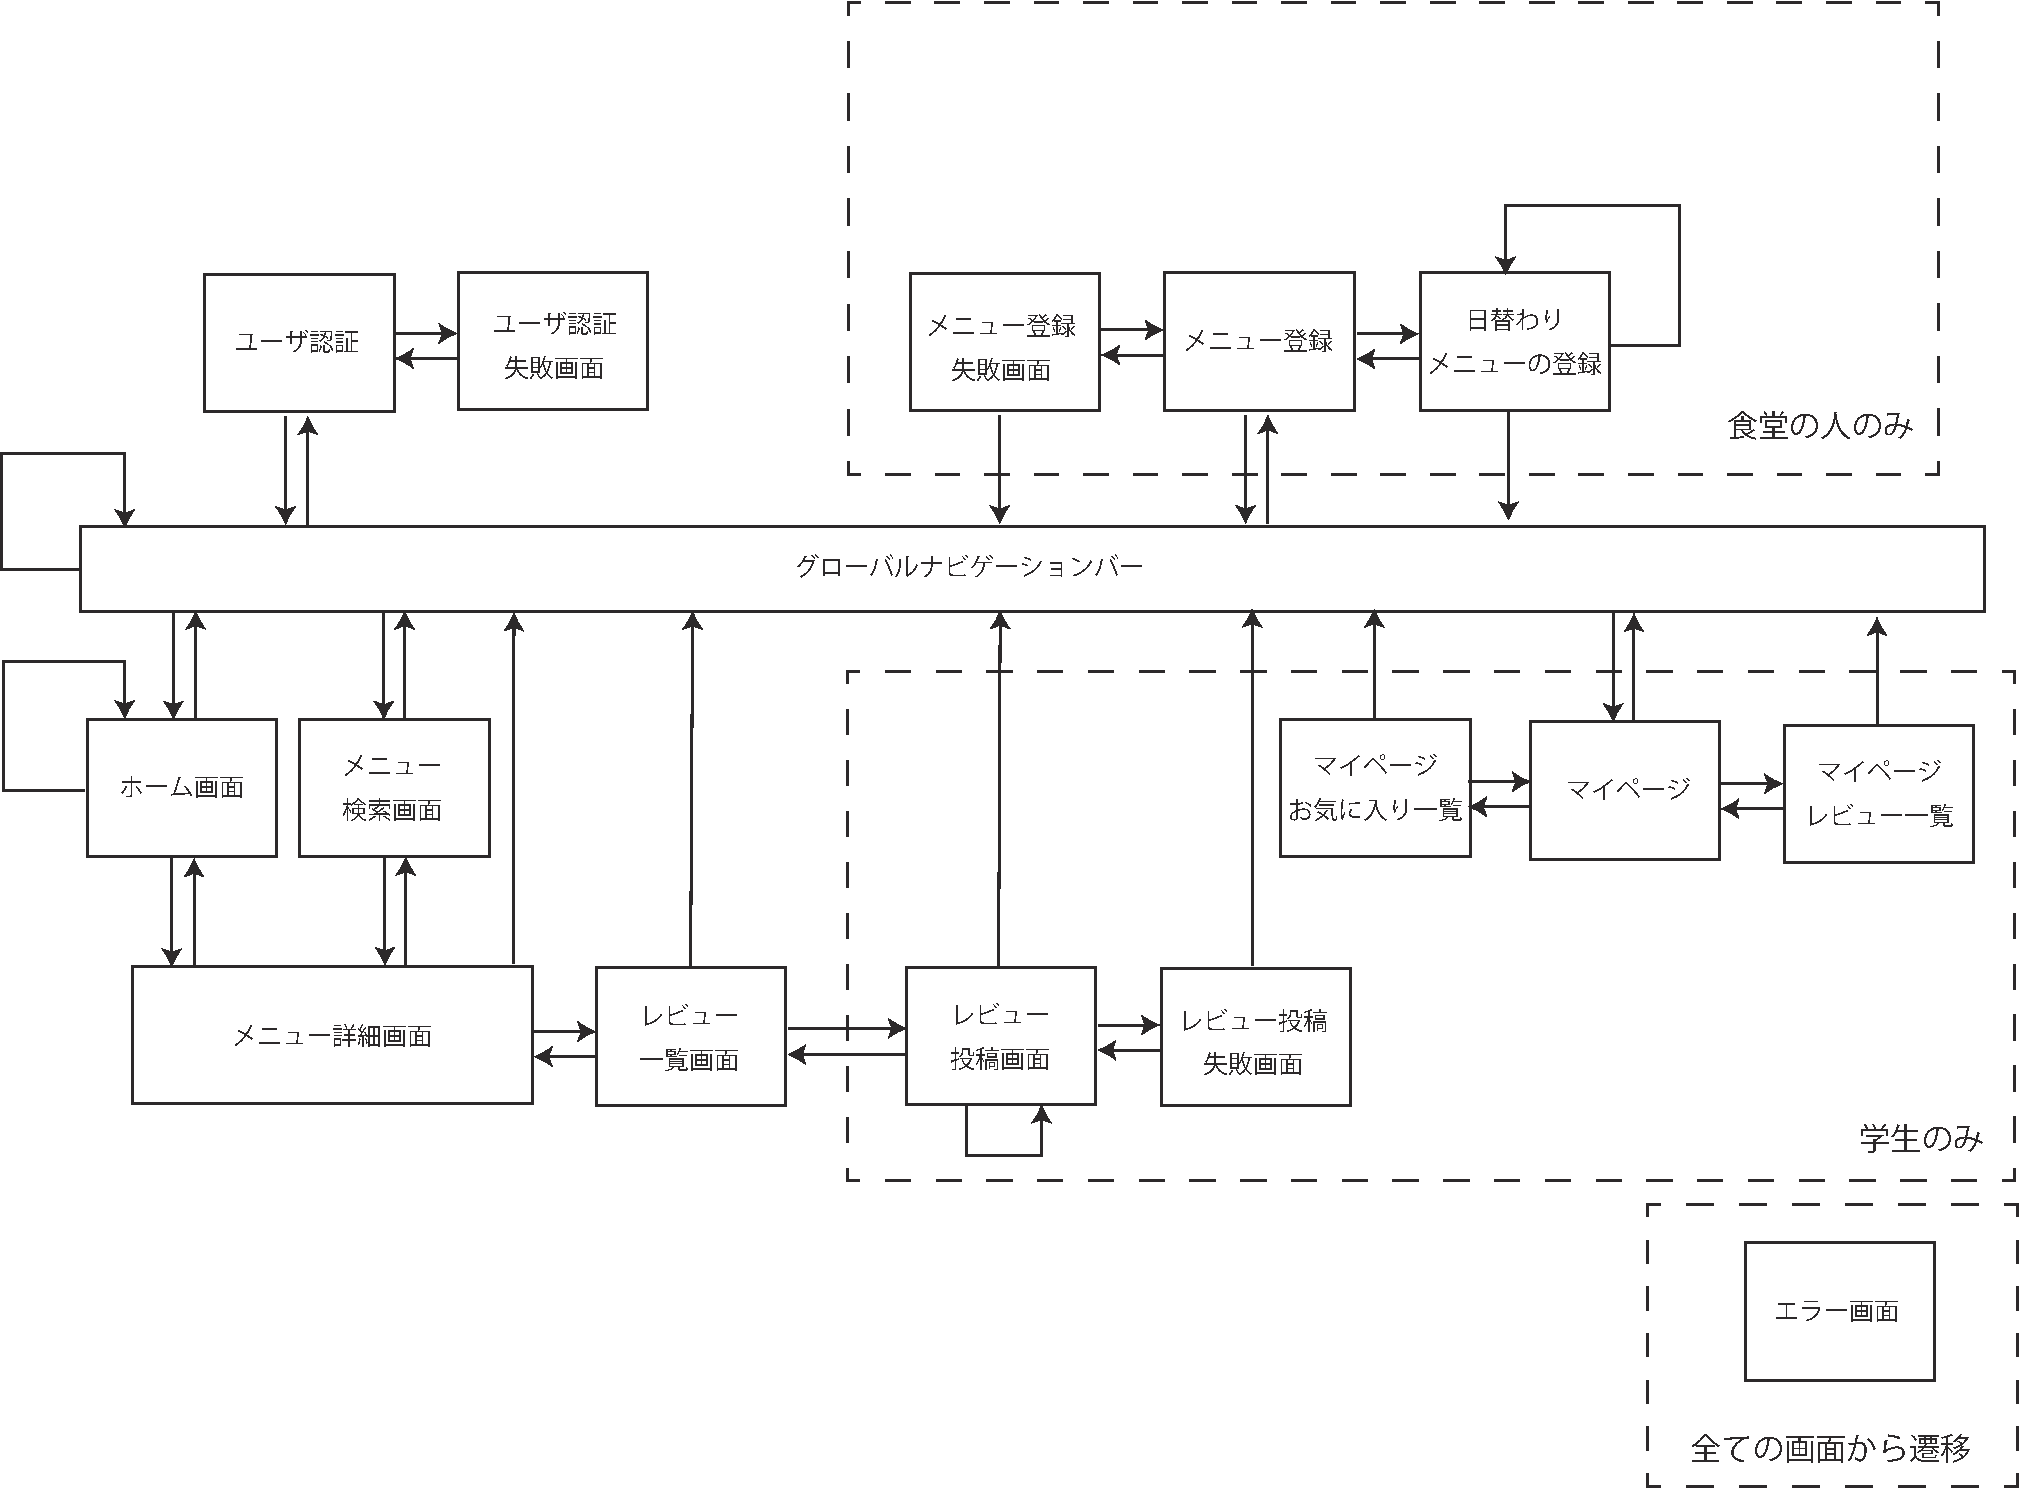
\includegraphics[width=145mm]{fig/transition.pdf}
            \caption{画面遷移図}
            \label{img:transition}
        \end{figure}
    \subsubsection{画面}
        図\ref{img:home-before-login}\sim\ref{img:review-list}に各画面を示す.
        \begin{figure}[ht]
            \begin{minipage}[t]{.49\textwidth}
                \center
                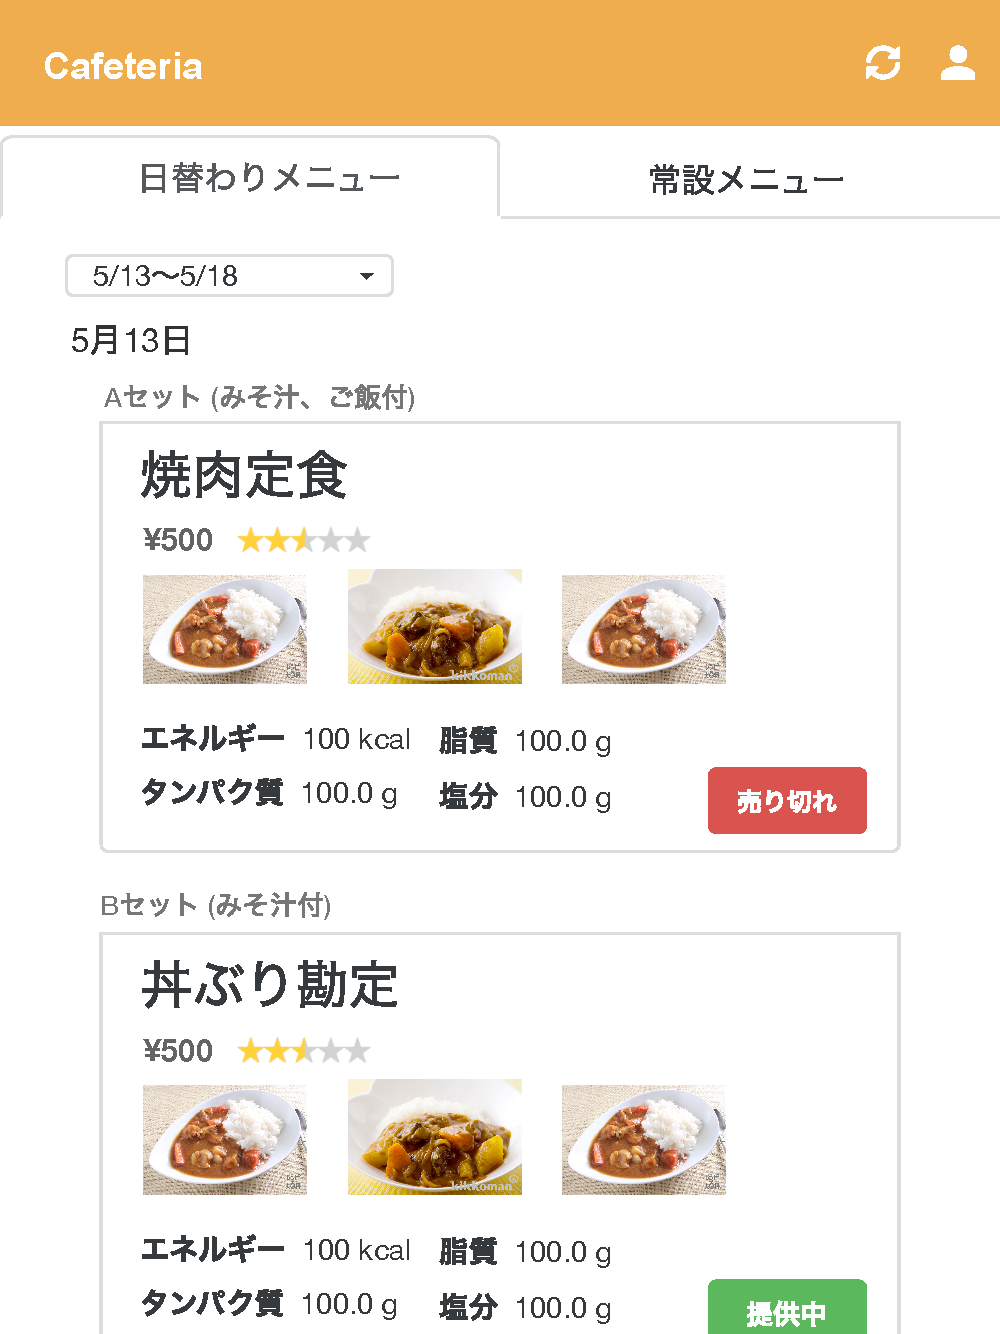
\includegraphics[width=60mm]{ui/home-before-login.png}
                \caption{ホーム画面(ログイン前)}
                \label{img:home-before-login}
            \end{minipage}
            \begin{minipage}[t]{.49\textwidth}
                \center
                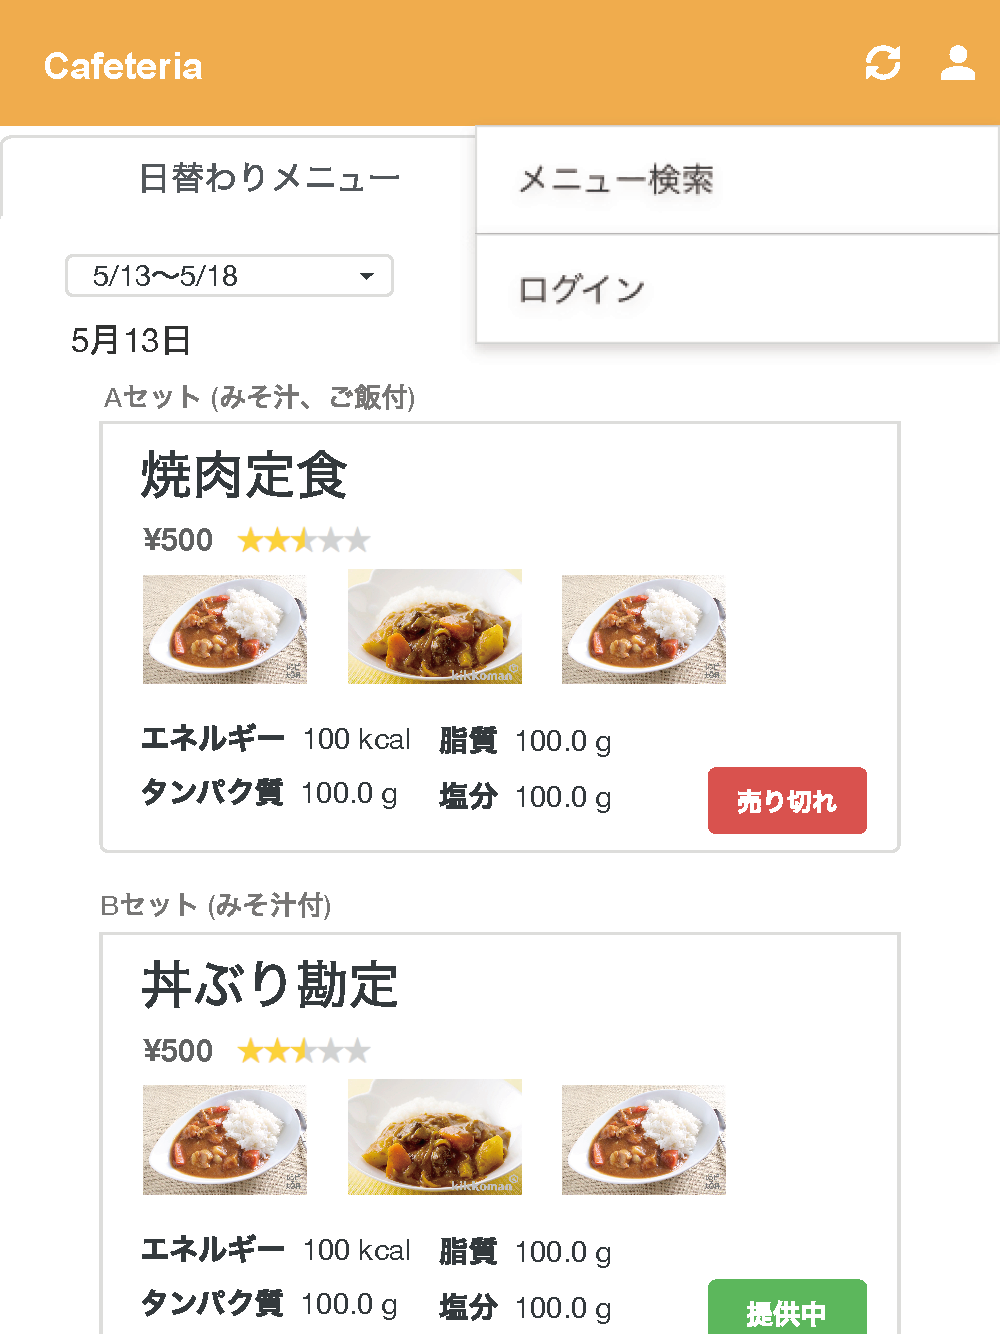
\includegraphics[width=60mm]{ui/home-dropdown-before-login.png}
                \caption{ホーム画面(ドロップダウン(ログイン前))}
                \label{img:home-dropdown-before-login}
            \end{minipage}
        \end{figure}
        \begin{figure}[ht]
            \begin{minipage}[t]{.49\textwidth}
                \center
                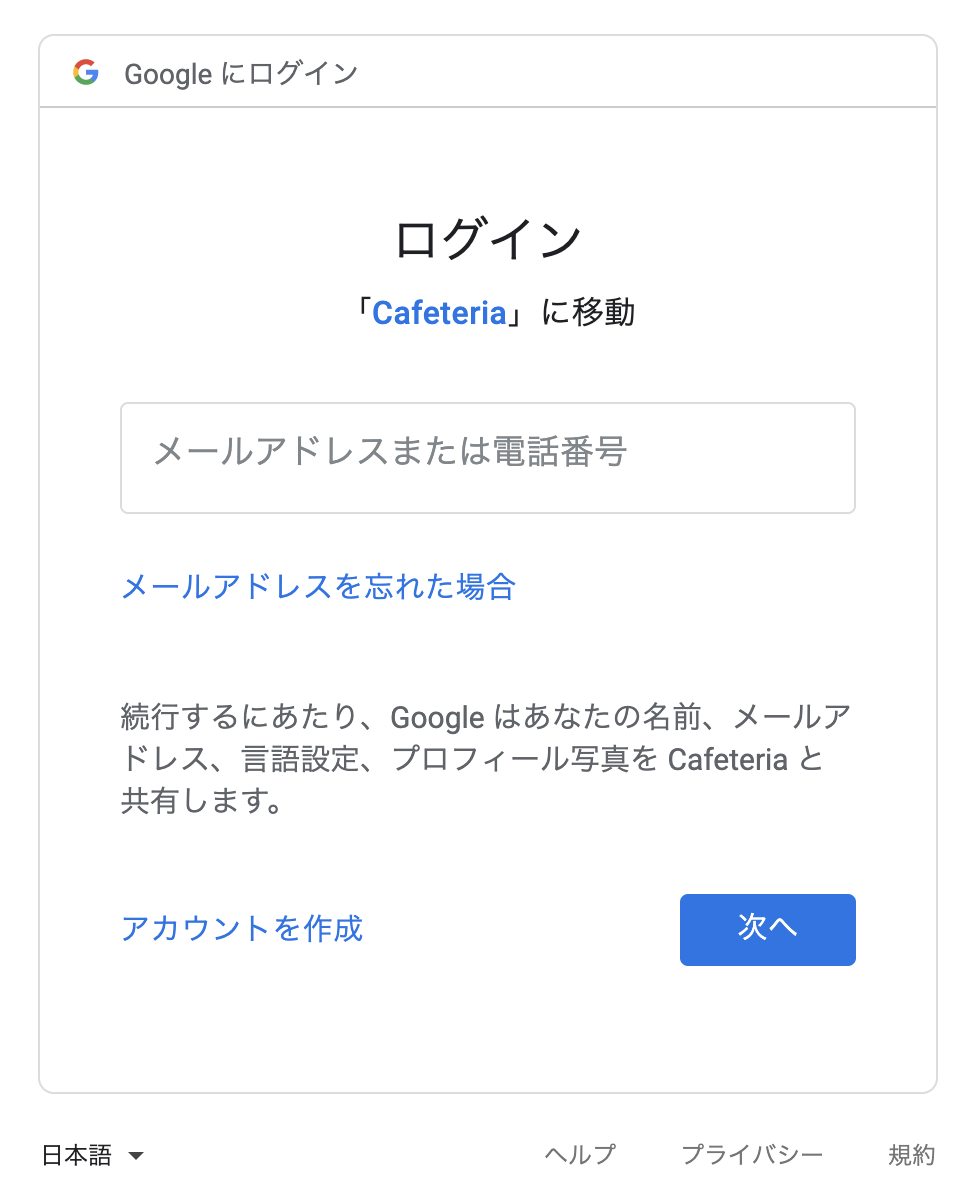
\includegraphics[width=60mm]{ui/login.png}
                \caption{ログイン画面}
                \label{img:login}
            \end{minipage}
            \begin{minipage}[t]{.49\textwidth}
                \center
                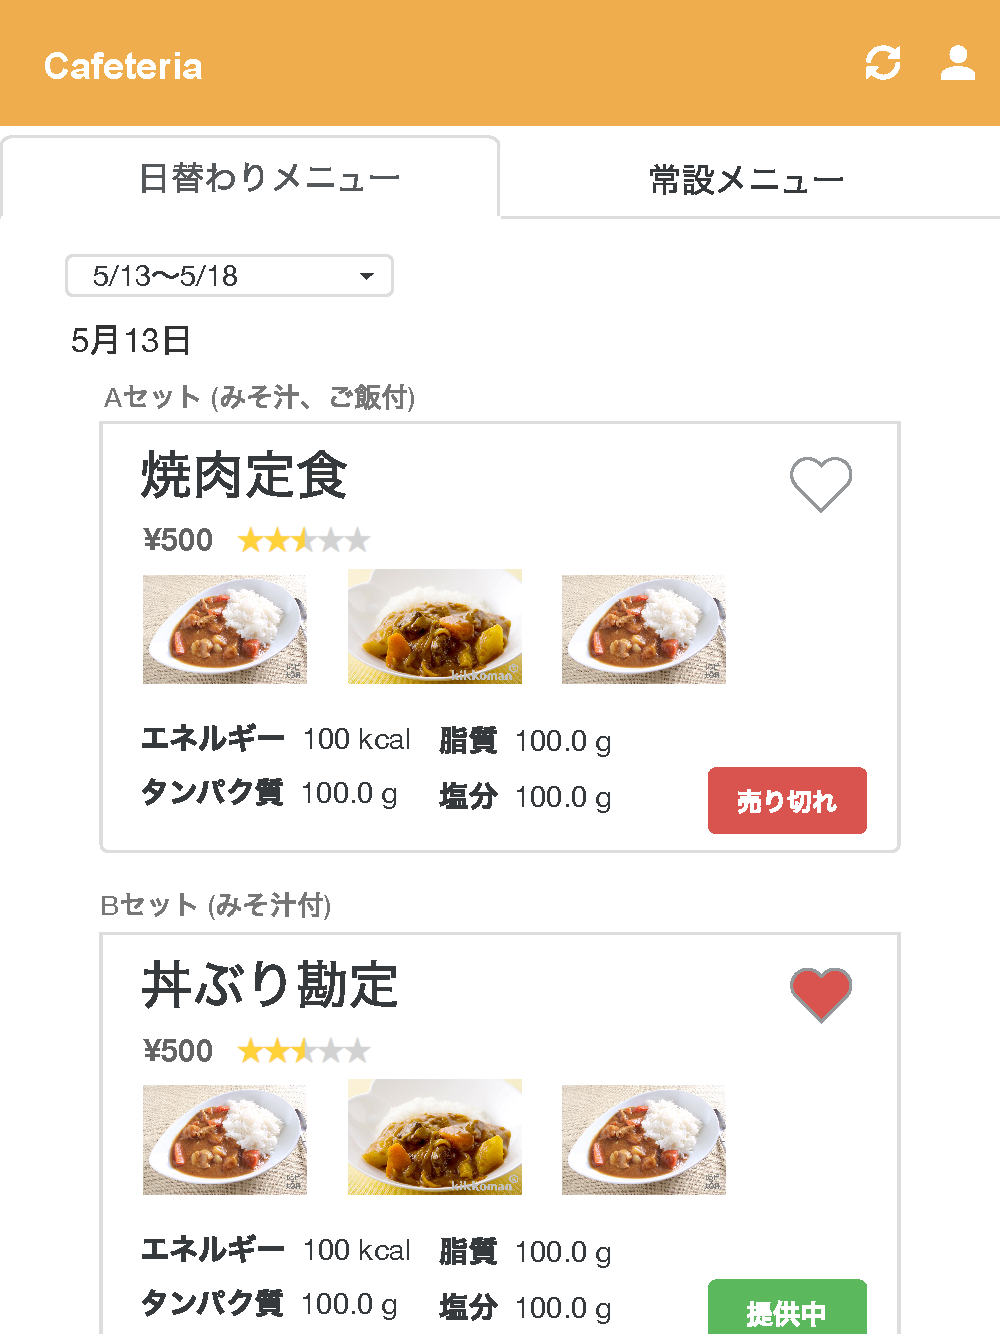
\includegraphics[width=60mm]{ui/home.png}
                \caption{ホーム画面(ログイン後)}
                \label{img:home}
            \end{minipage}
        \end{figure}
        \begin{figure}[ht]
            \begin{minipage}[t]{.49\textwidth}
                \center
                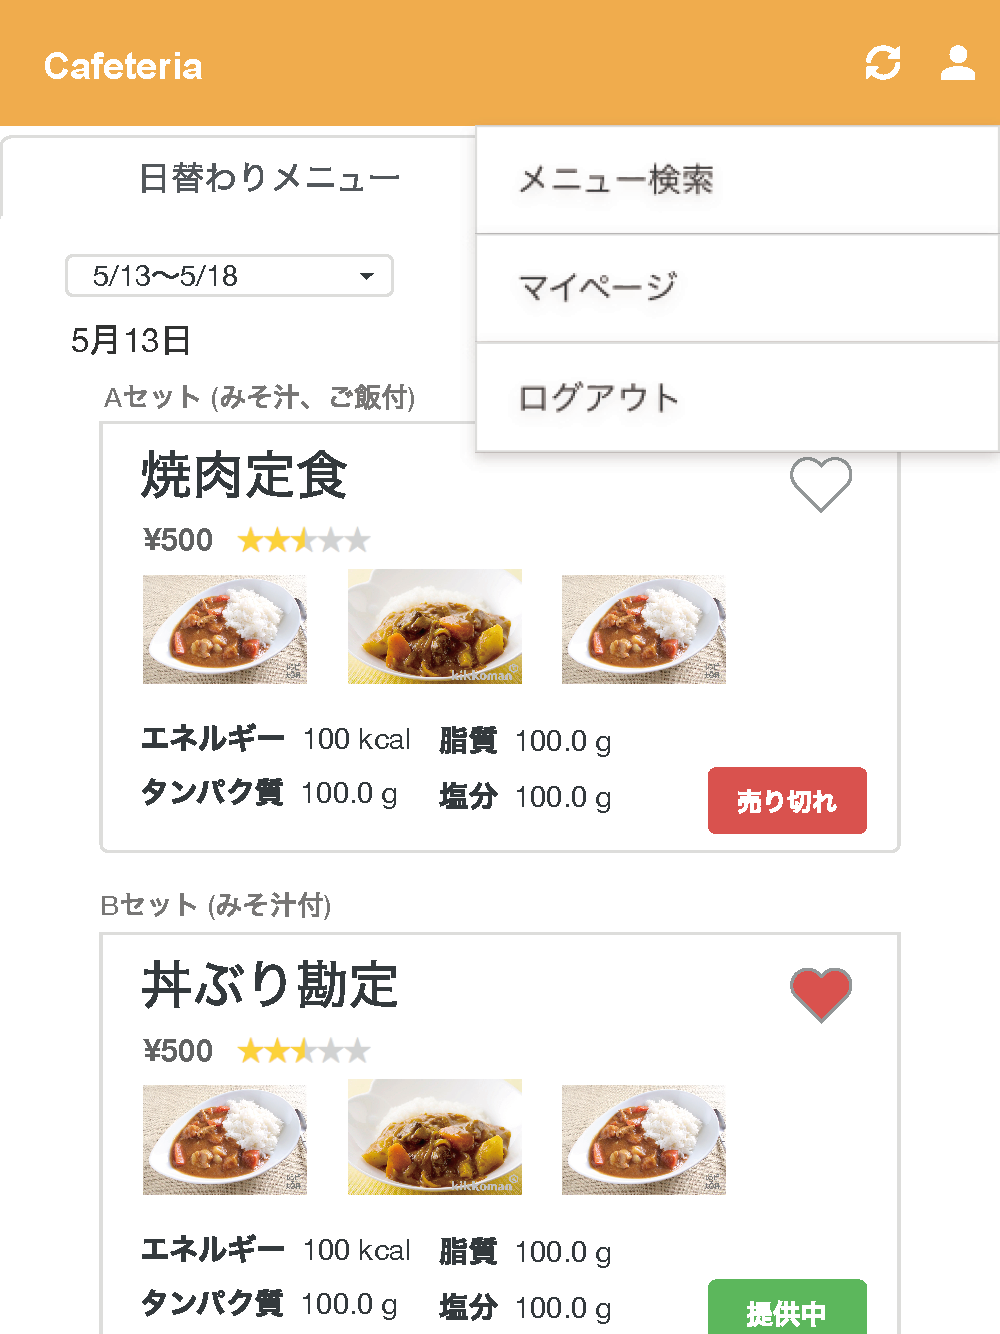
\includegraphics[width=60mm]{ui/home-dropdown.png}
                \caption{ホーム画面(ドロップダウン(ログイン後))}
                \label{img:home-dropdown}
            \end{minipage}
            \begin{minipage}[t]{.49\textwidth}
                \center
                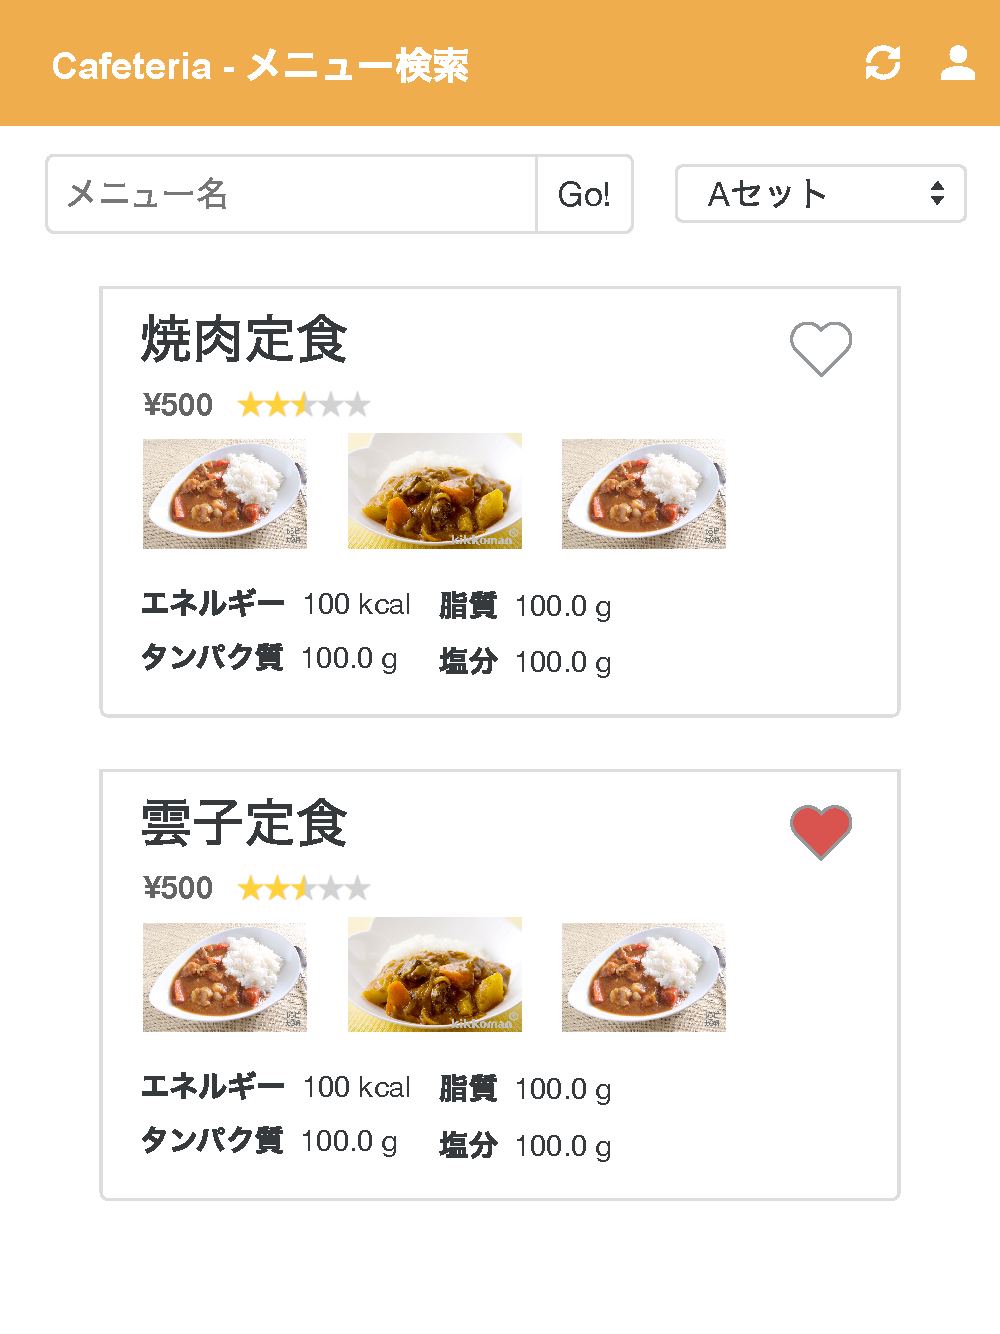
\includegraphics[width=60mm]{ui/menu-search.png}
                \caption{メニュー検索画面}
                \label{img:menu-search}
            \end{minipage}
        \end{figure}
        \begin{figure}[ht]
            \begin{minipage}[t]{.49\textwidth}
                \center
                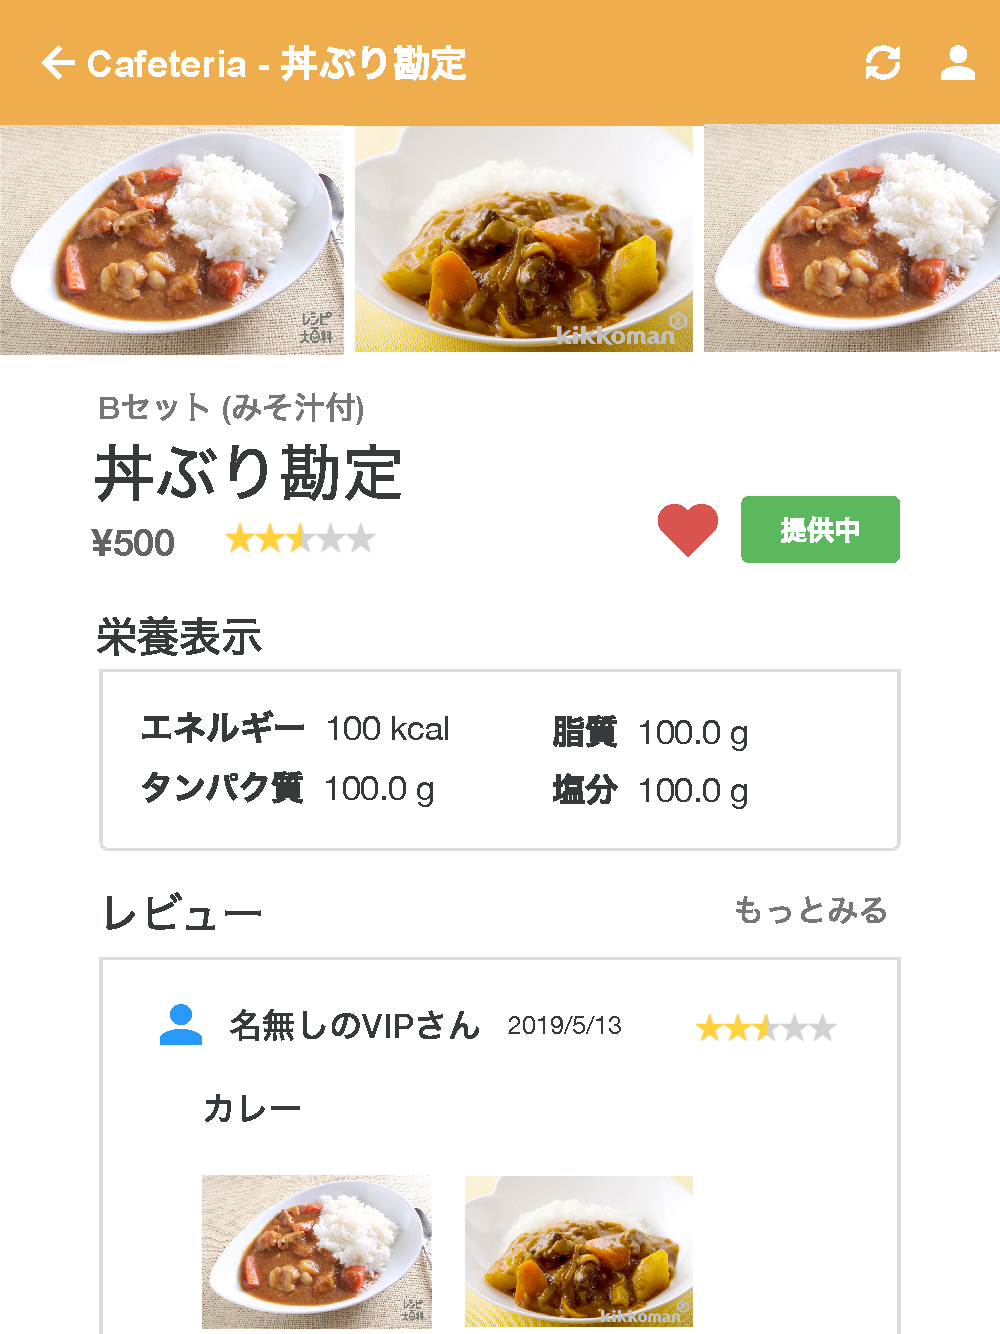
\includegraphics[width=60mm]{ui/detail-head.png}
                \caption{メニュー詳細画面}
                \label{img:detail-head}
            \end{minipage}
            \begin{minipage}[t]{.49\textwidth}
                \center
                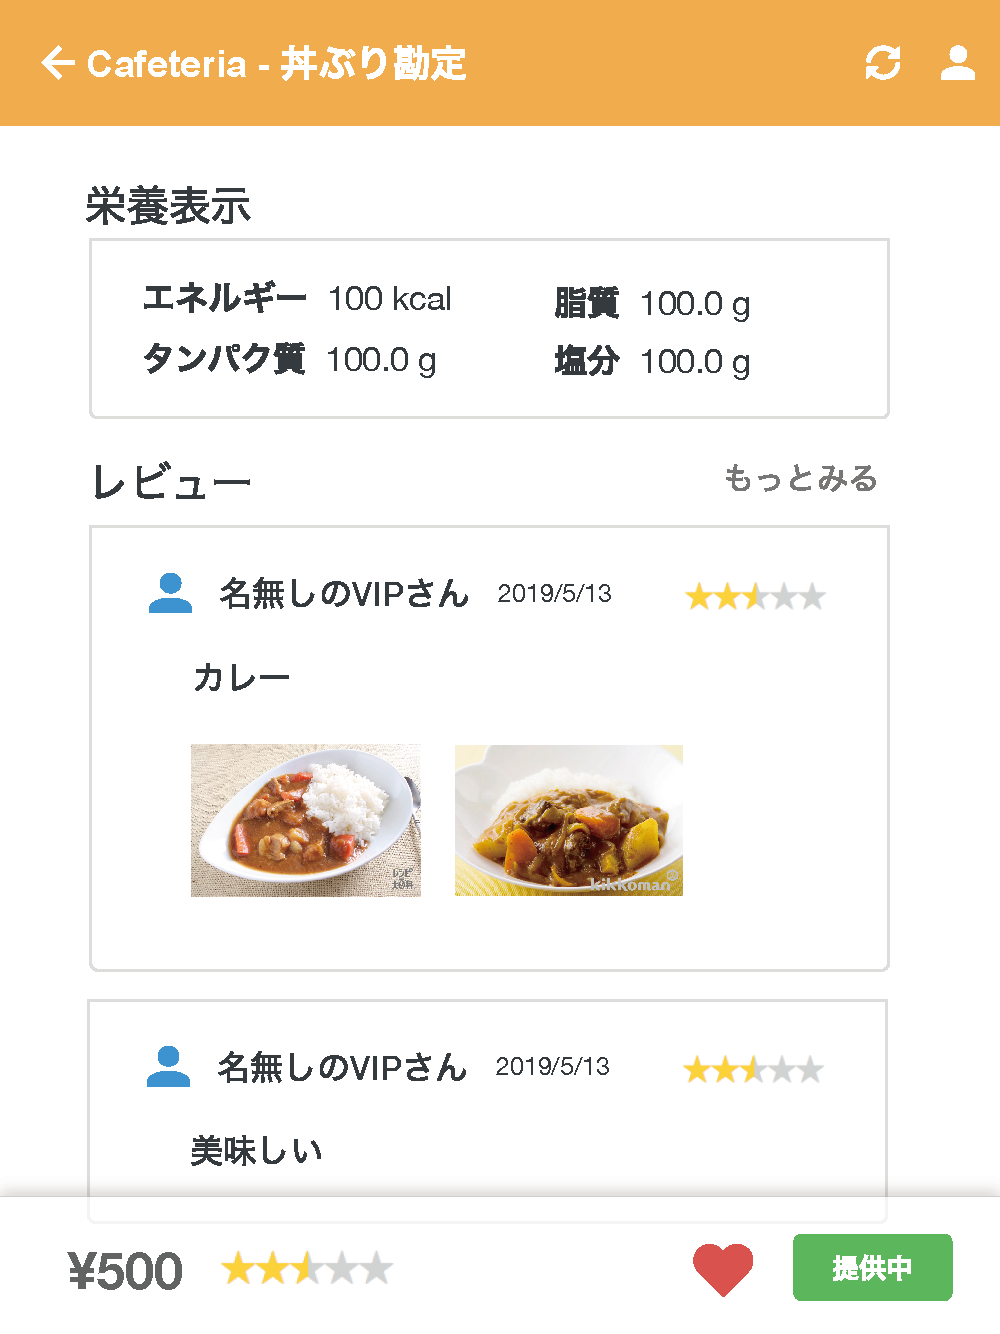
\includegraphics[width=60mm]{ui/detail-tail.png}
                \caption{メニュー詳細画面(スクロール)}
                \label{img:detail-tail}
            \end{minipage}
        \end{figure}
        \begin{figure}[ht]
            \begin{minipage}[t]{.49\textwidth}
                \center
                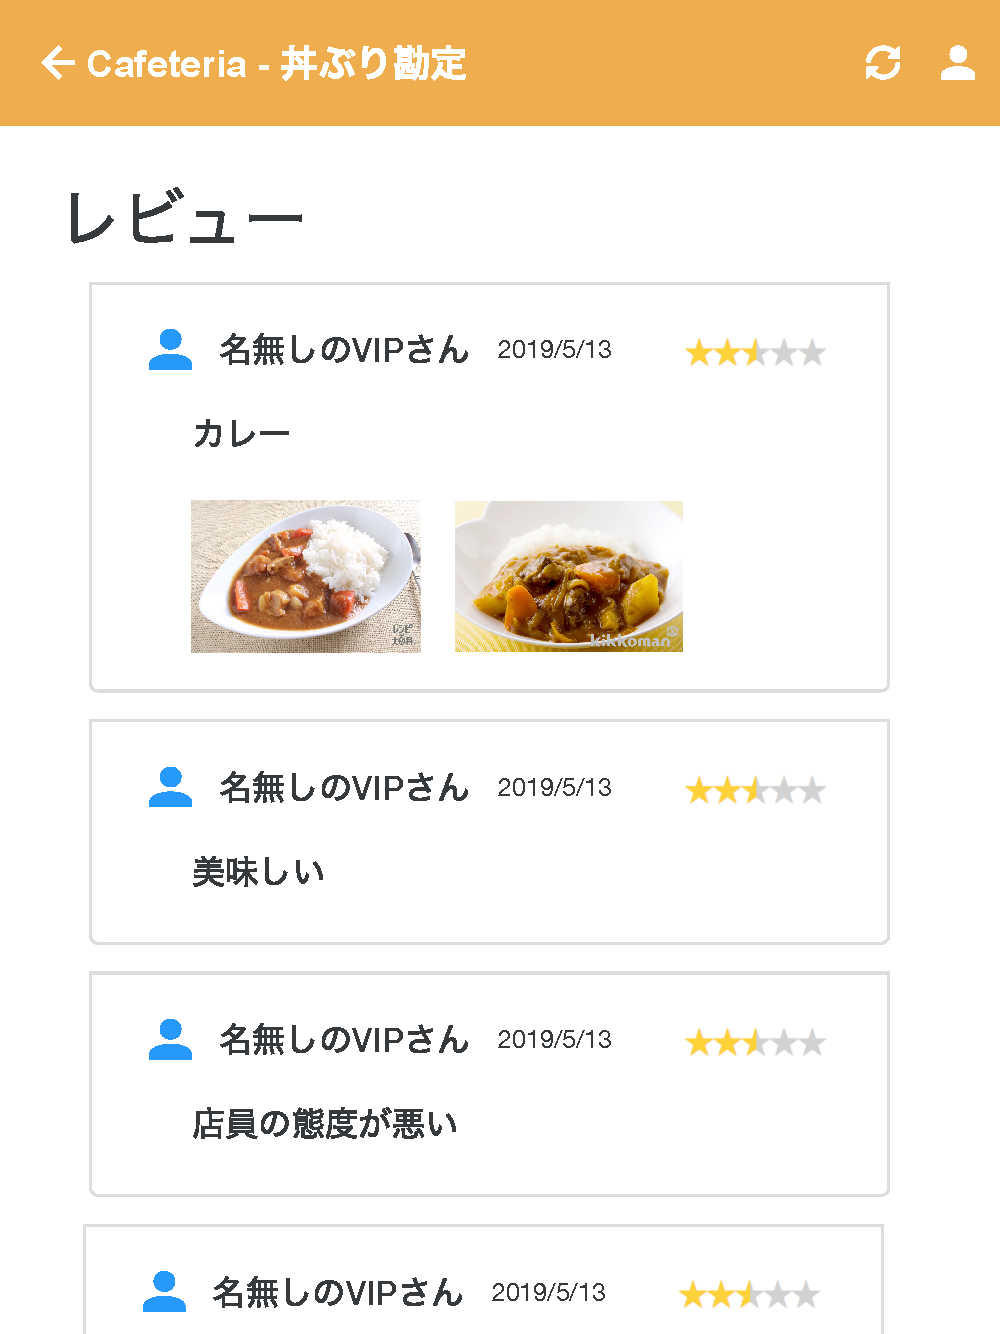
\includegraphics[width=60mm]{ui/detail-review.png}
                \caption{レビュー詳細画面}
                \label{img:detail-review}
            \end{minipage}
            \begin{minipage}[t]{.49\textwidth}
                \center
                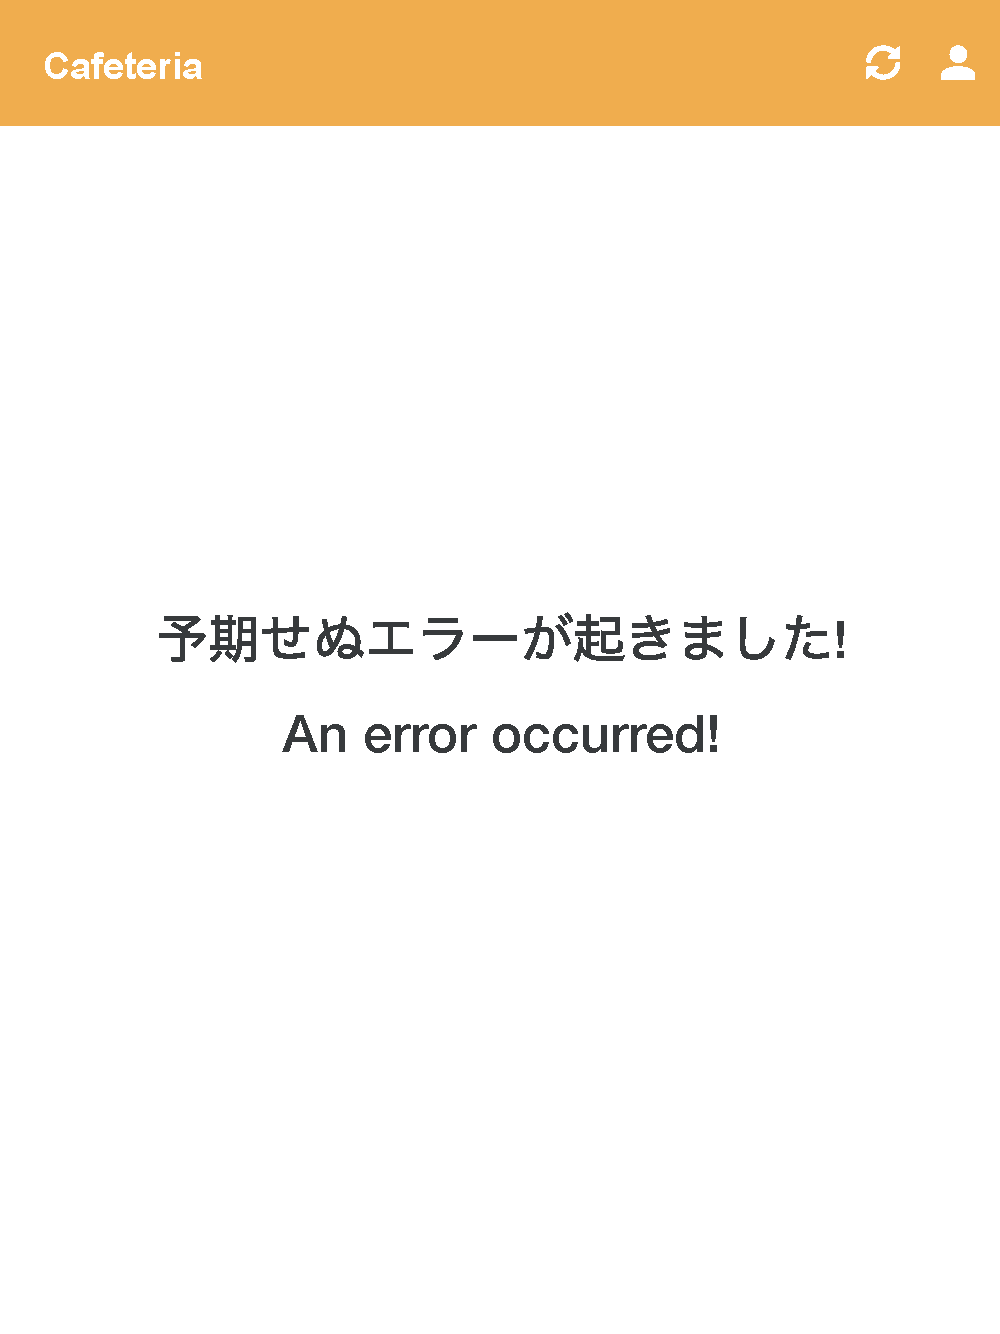
\includegraphics[width=60mm]{ui/error.png}
                \caption{エラー画面}
                \label{img:error}
            \end{minipage}
        \end{figure}
        \begin{figure}[ht]
            \begin{minipage}[t]{.49\textwidth}
                \center
                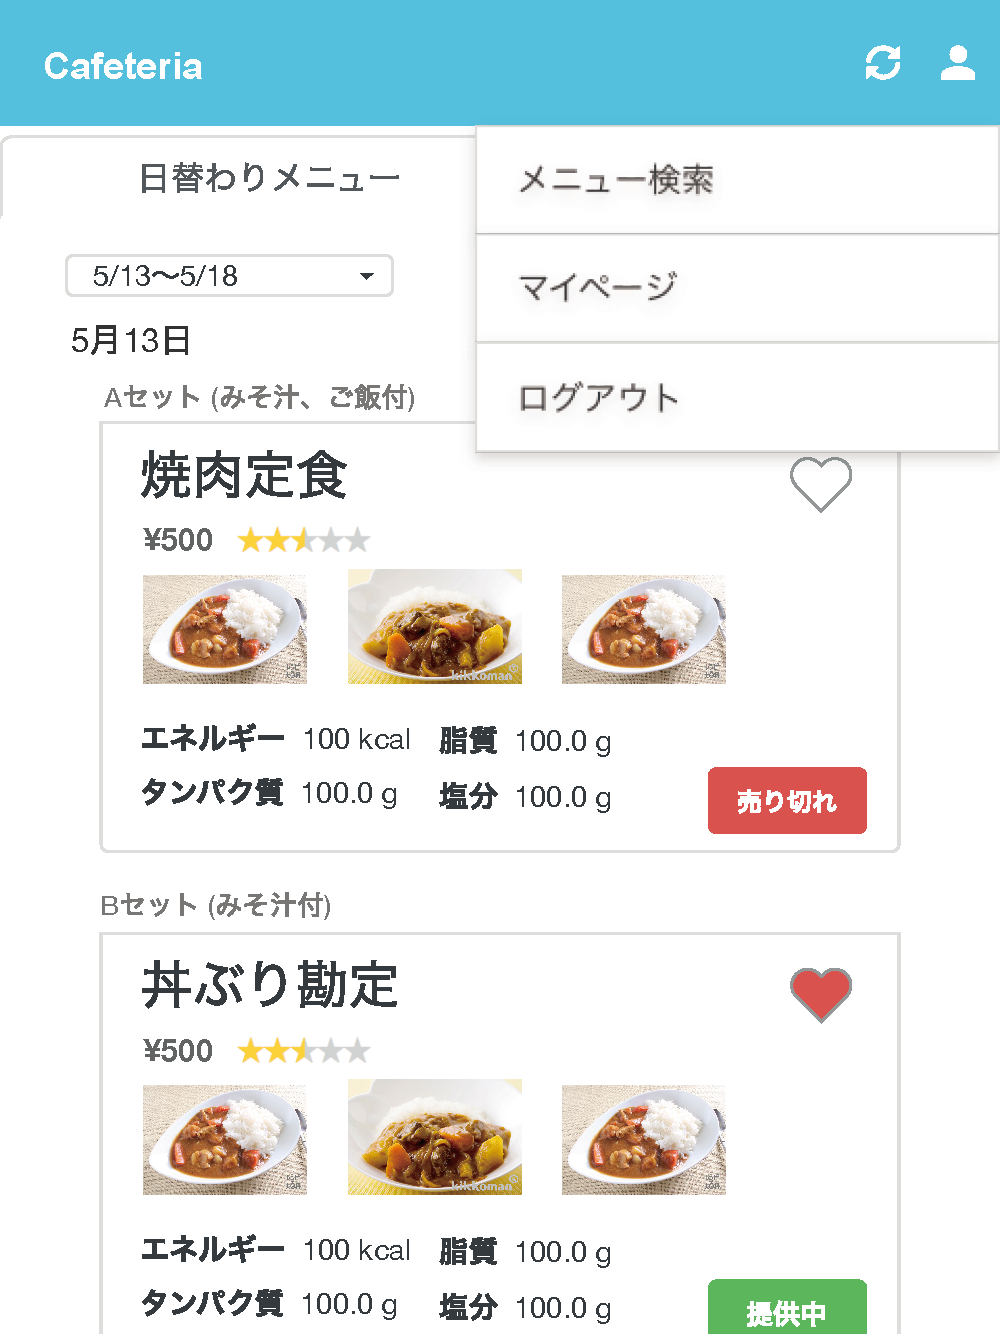
\includegraphics[width=60mm]{ui/admin-home-dropdown.png}
                \caption{管理者画面}
                \label{img:admin-home-dropdown}
            \end{minipage}
            \begin{minipage}[t]{.49\textwidth}
                \center
                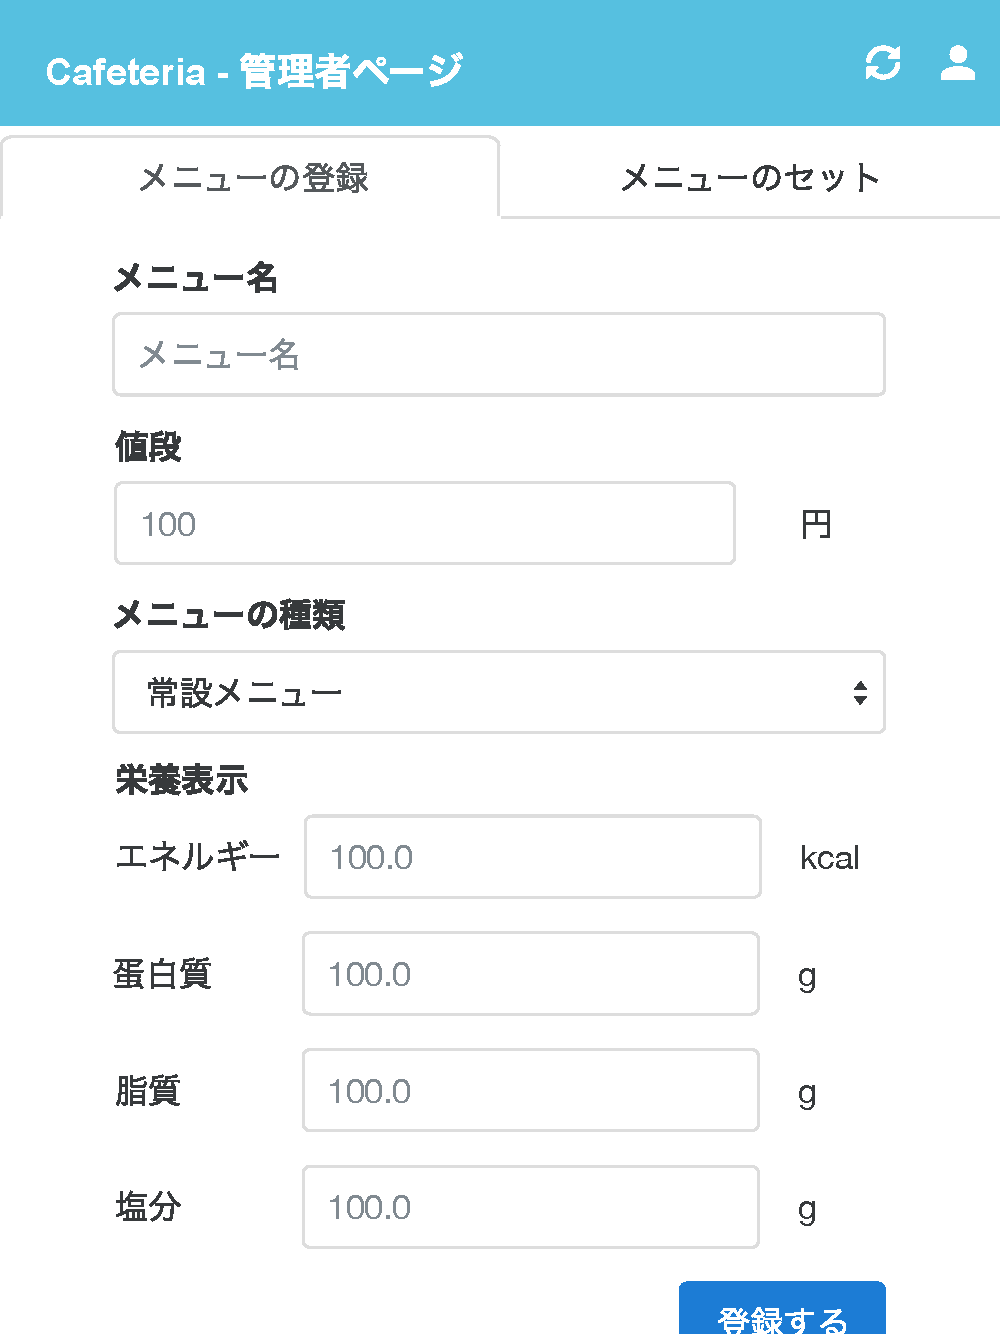
\includegraphics[width=60mm]{ui/admin-home-new-menu.png}
                \caption{管理者画面(メニュー追加 )}
                \label{img:admin-home-new-menu}
            \end{minipage}
        \end{figure}
        \begin{figure}[ht]
            \begin{minipage}[t]{.49\textwidth}
                \center
                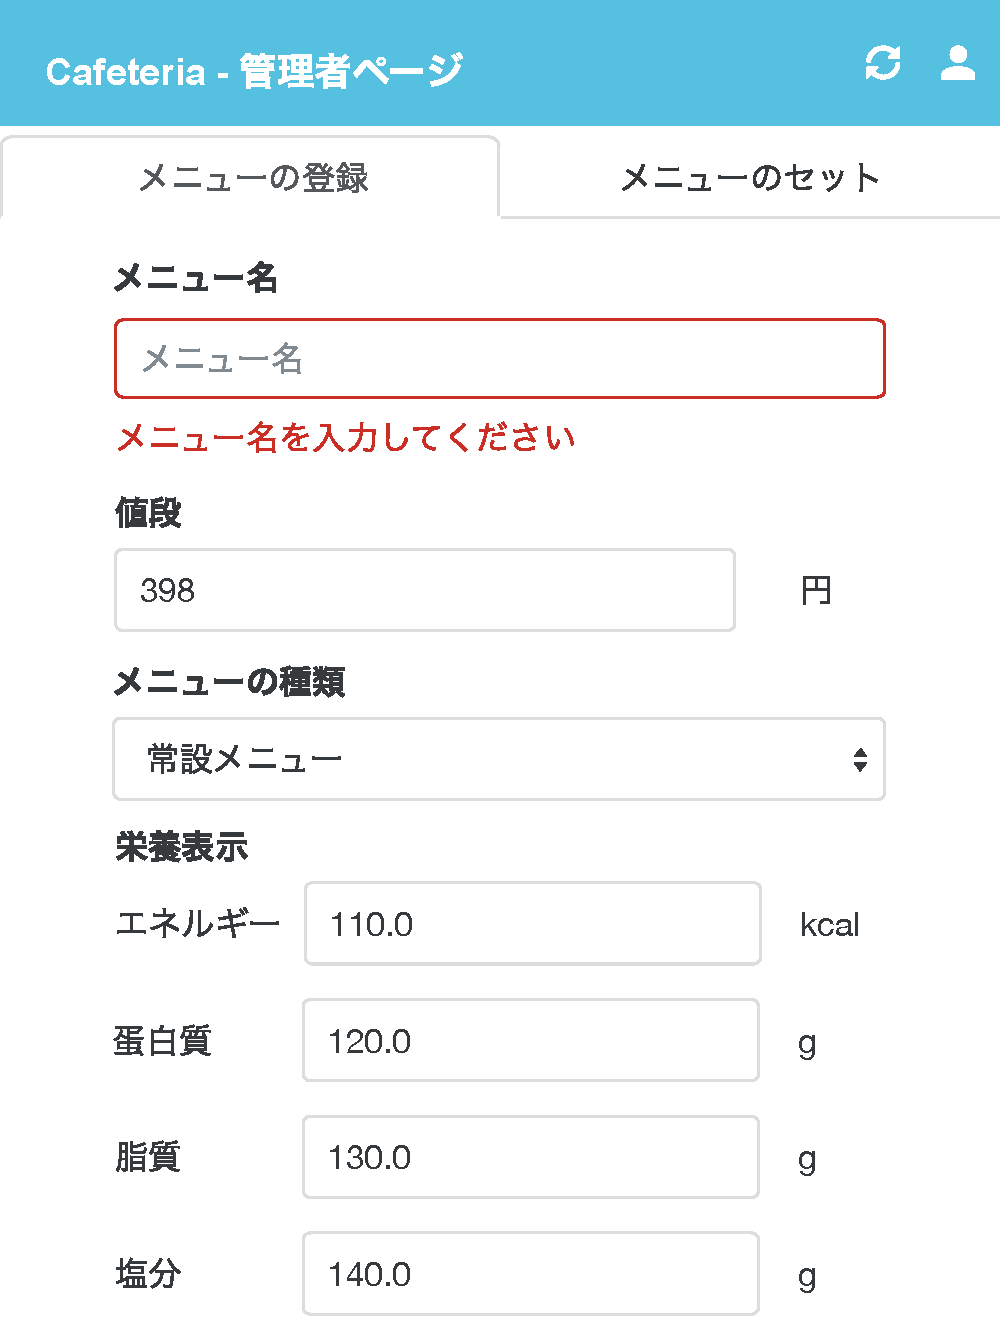
\includegraphics[width=60mm]{ui/admin-home-new-menu-error.png}
                \caption{管理者画面(メニュー追加(エラー))}
                \label{img:admin-home-new-menu-error}
            \end{minipage}
            \begin{minipage}[t]{.49\textwidth}
                \center
                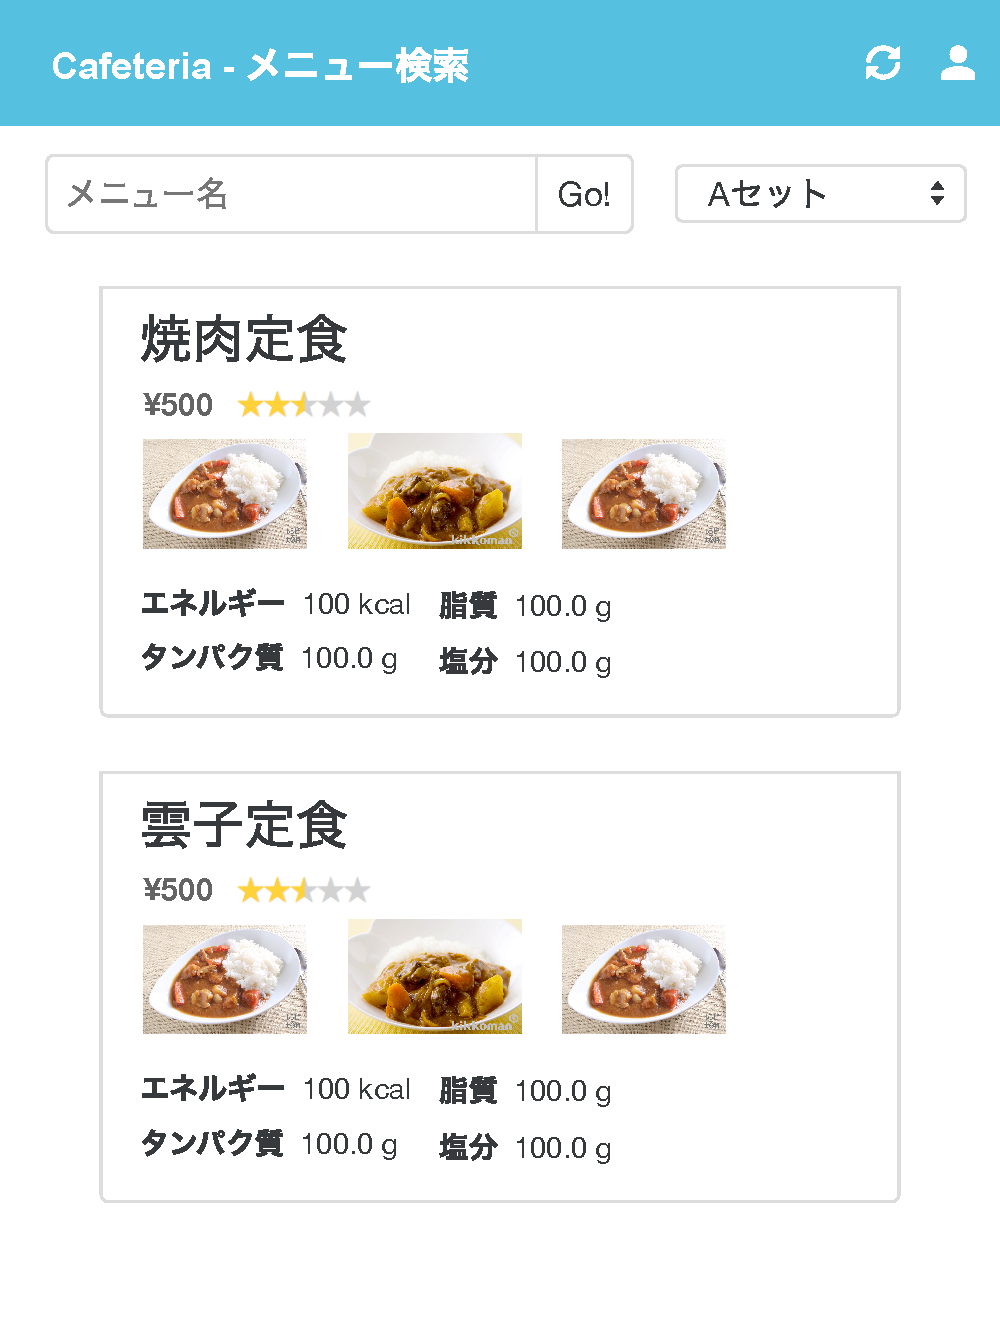
\includegraphics[width=60mm]{ui/admin-menu-search.png}
                \caption{管理者画面(メニュー検索)}
                \label{img:admin-menu-search}
            \end{minipage}
        \end{figure}
        \begin{figure}[ht]
            \begin{minipage}[t]{.49\textwidth}
                \center
                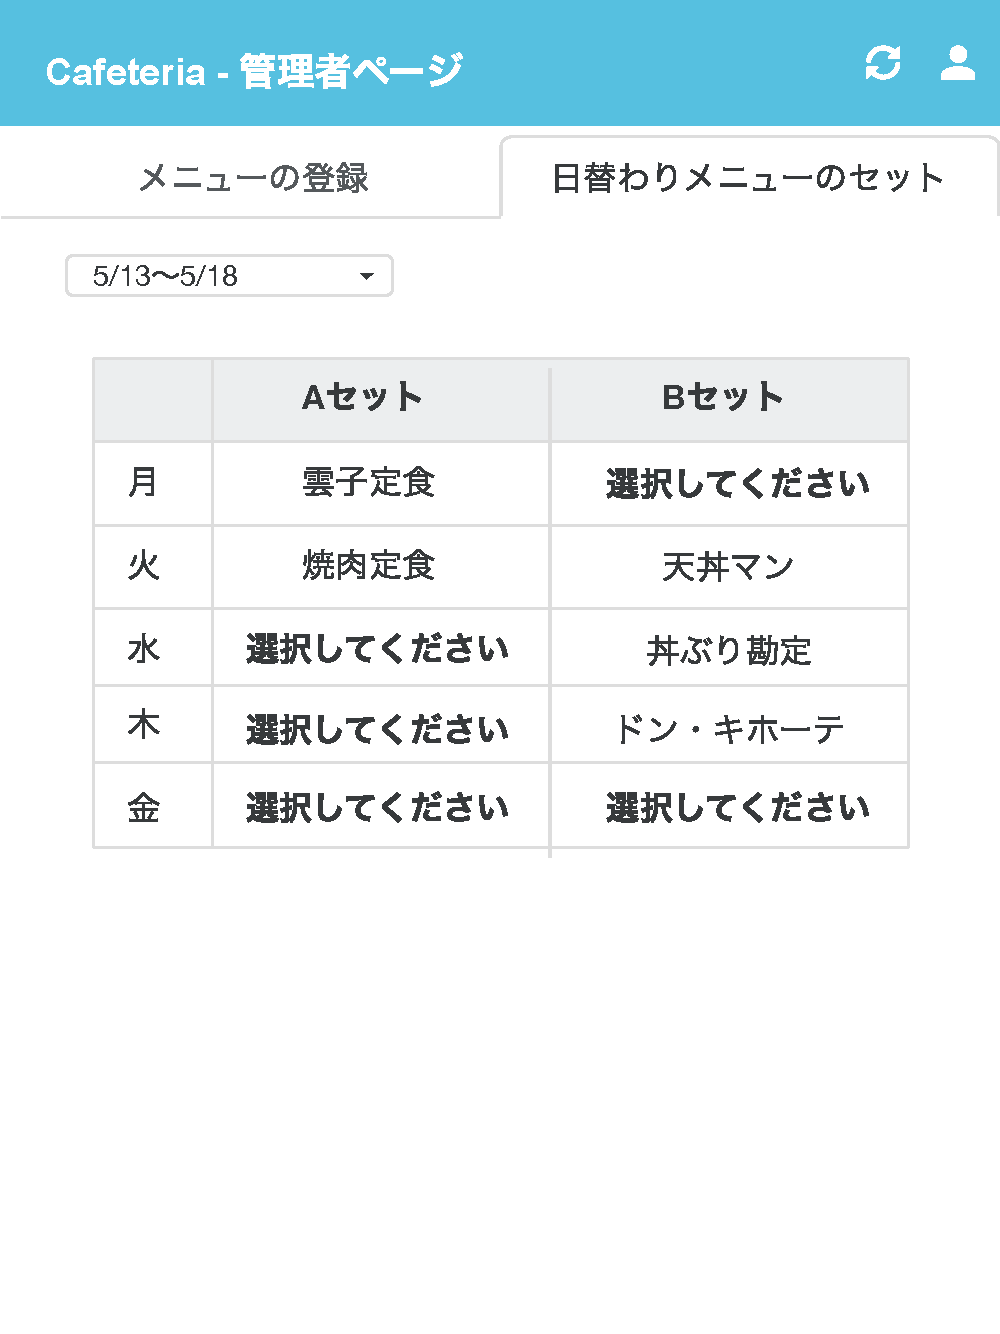
\includegraphics[width=60mm]{ui/admin-home-set-menu.png}
                \caption{管理者画面(日替わりメニュー登録)}
                \label{img:admin-home-set-menu}
            \end{minipage}
            \begin{minipage}[t]{.49\textwidth}
                \center
                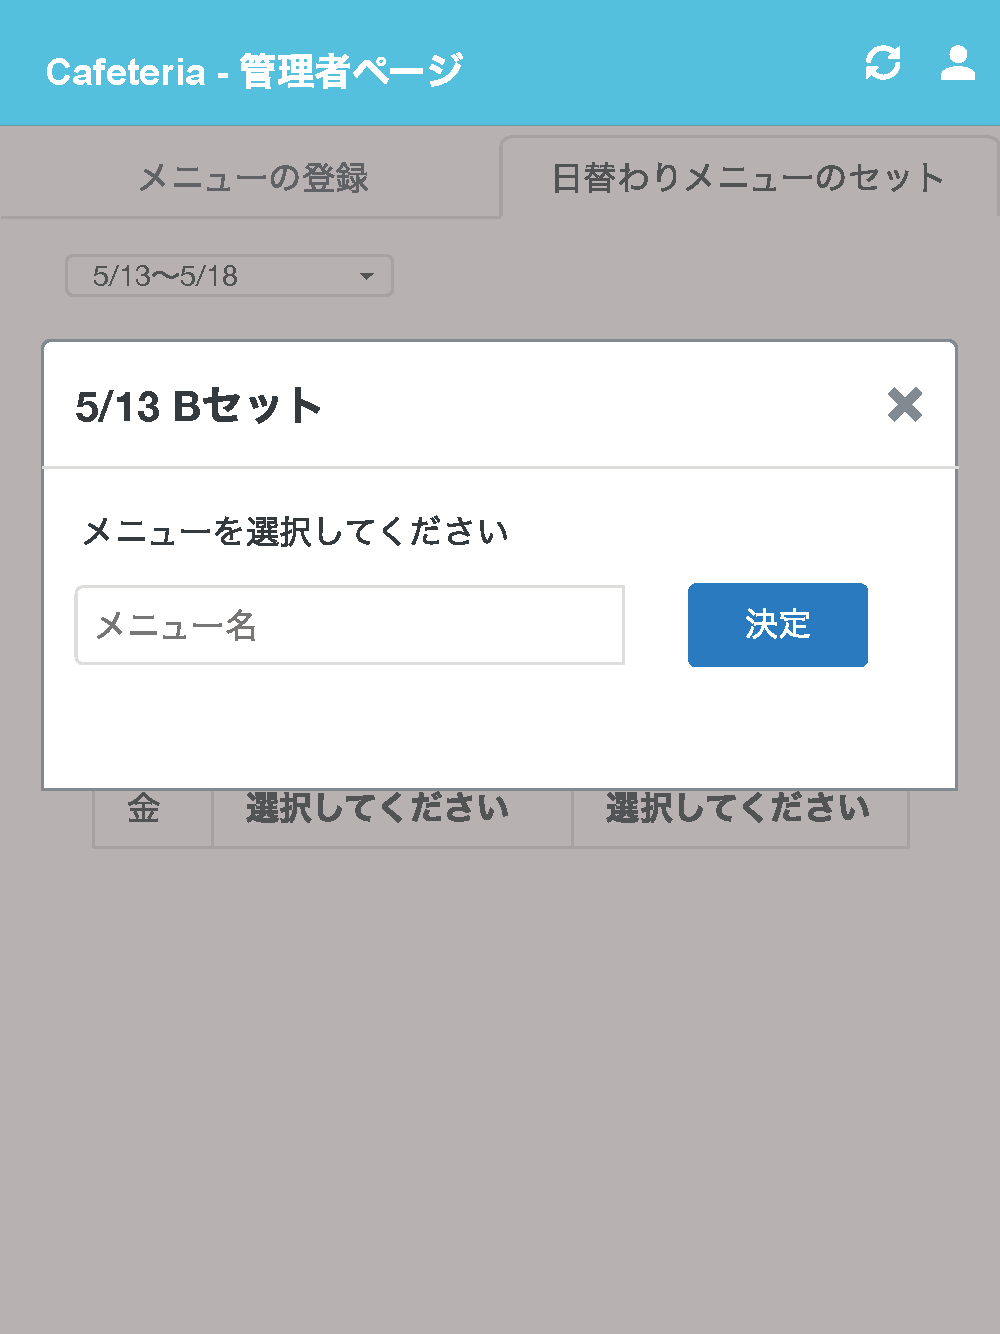
\includegraphics[width=60mm]{ui/admin-home-set-menu-modal.png}
                \caption{管理者画面(メニュー変更モーダル)}
                \label{img:admin-home-set-menu-modal}
            \end{minipage}
        \end{figure}
        \begin{figure}[ht]
            \begin{minipage}[t]{.49\textwidth}
                \center
                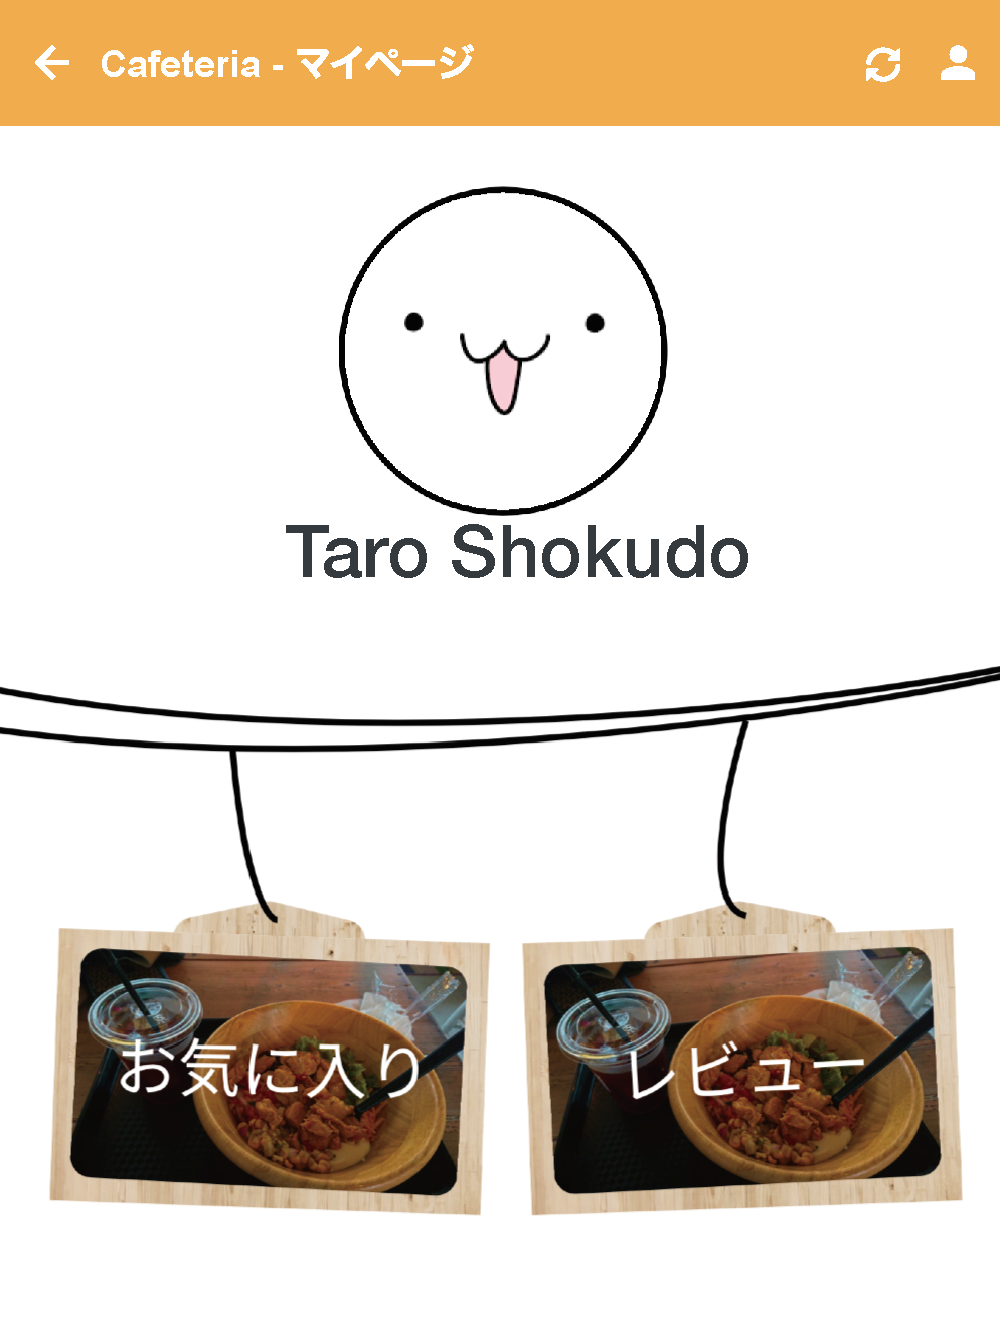
\includegraphics[width=60mm]{ui/my-page.png}
                \caption{マイページ}
                \label{img:my-page}
            \end{minipage}
            \begin{minipage}[t]{.49\textwidth}
                \center
                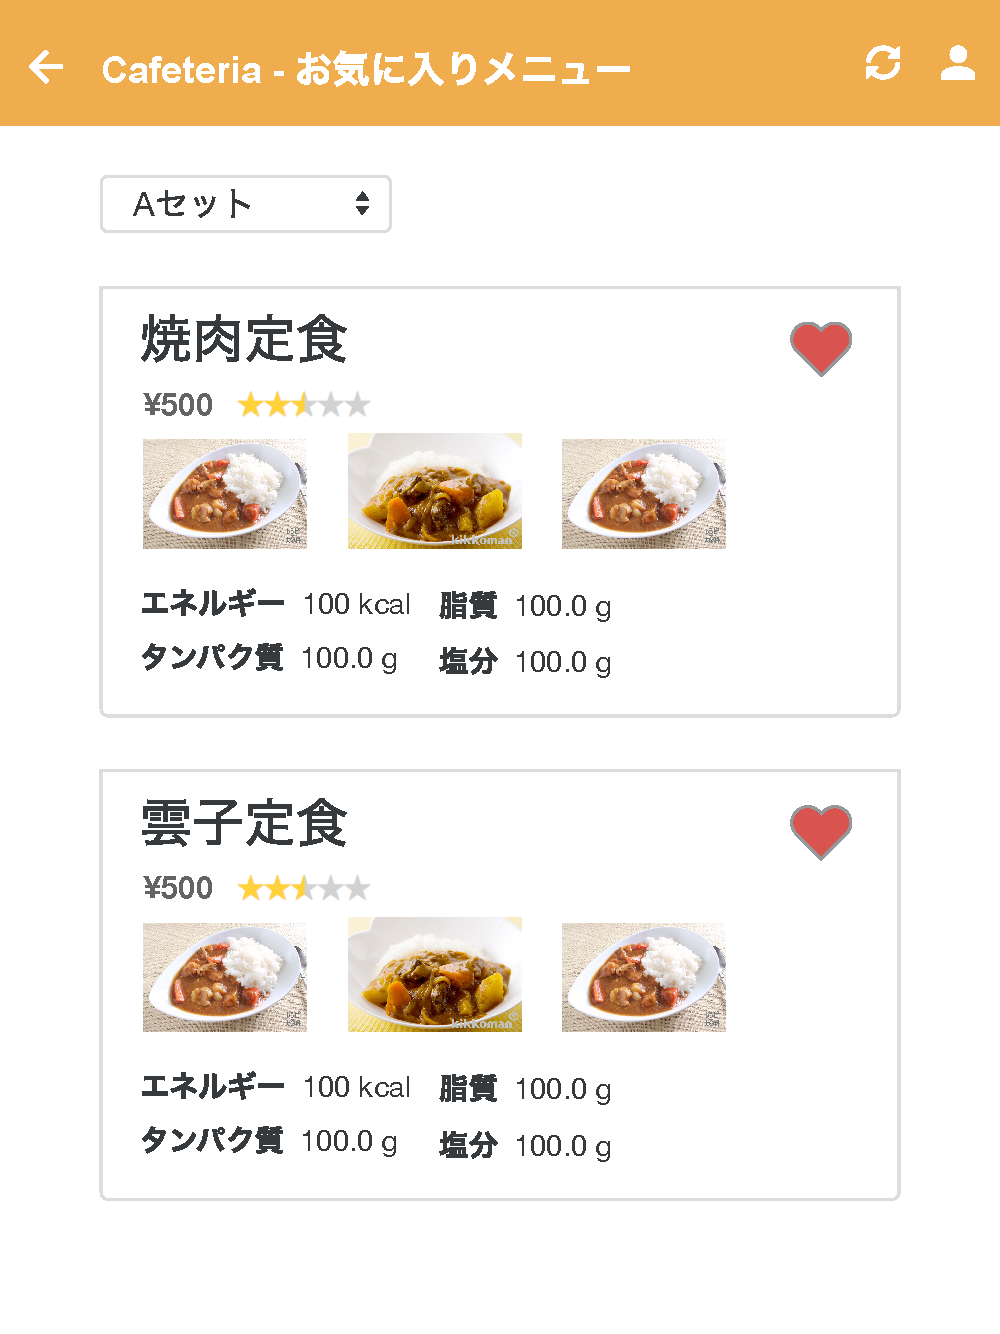
\includegraphics[width=60mm]{ui/liked-list.png}
                \caption{マイページ(お気に入り一覧)}
                \label{img:liked-list}
            \end{minipage}
        \end{figure}
        \begin{figure}[ht]
            \center
            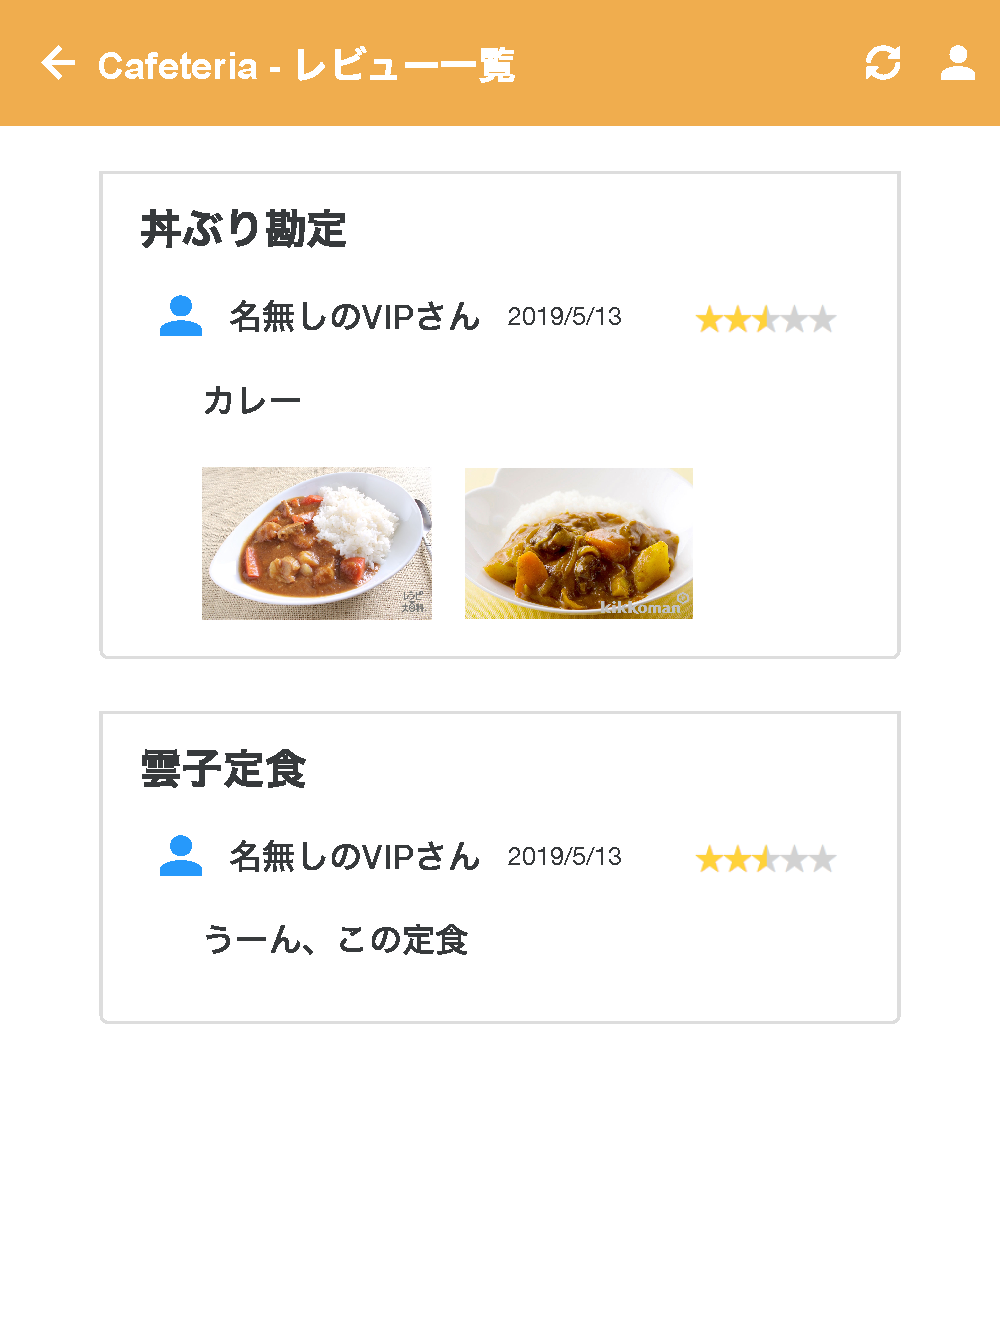
\includegraphics[width=60mm]{ui/review-list.png}
            \caption{マイページ(レビュー一覧)}
            \label{img:review-list}
        \end{figure}

\clearpage

\section{内部設計}
    \subsection{サーバサイド技術}
        サーバサイド技術はPHP\,7.0を使用し,フレームワークとしてLaravel\,5.5を使用する.
        そのため,\, PHP拡張モジュールとして以下が必要となる.
        \begin{itemize}
            \item OpenSSL PHP Extension
            \item PDO PHP Extension
            \item Mbstring PHP Extension
            \item Tokenizer PHP Extension
            \item XML PHP Extension
            \item JSON PHP Extension
            \item PostgreSQL PHP Extension
        \end{itemize}
    \subsection{データベース}
        データベースのテーブルを表\ref{daily-menu}\sim\ref{users}に示す.
        \begin{table}[h]
            \begin{minipage}[t]{.49\textwidth}
                \center
                \caption{日替わりメニュー}
                \label{daily-menu}
                \begin{tabular}{|c|c|}
                    \hline
                    \multicolumn{2}{|c|}{\texttt{daily\_menu}} \\ \hline \hline
                    \verb|date| & \verb|DATE| \\ \Hline
                    \verb|menu_id_A| & \verb|INTEGER| \\ \hline
                    \verb|menu_id_B| & \verb|INTEGER| \\ \hline
                \end{tabular}
                \center
                \caption{売り切れ}
                \label{soldout}
                \begin{tabular}{|c|c|}
                    \hline
                    \multicolumn{2}{|c|}{\texttt{sold\_out}} \\ \hline \hline
                    \verb|menu_id| & \verb|INTEGER| \\ \Hline
                    \verb|sold_out| & \verb|BOOLEAN| \\ \hline
                    \verb|created_at| & \verb|TIMESTAMP| \\ \hline
                    \verb|updated_at| & \verb|TIMESTAMP| \\ \hline
                \end{tabular}
            \end{minipage}
            \begin{minipage}[t]{.49\textwidth}
                \center
                \caption{メニュー}
                \label{menu}
                \begin{tabular}{|c|c|}
                    \hline
                    \multicolumn{2}{|c|}{\texttt{menus}} \\ \hline \hline
                    \verb|menu_id| & \verb|BIGINT| \\ \Hline
                    \verb|item_name| & \verb|VARCHAR(255)| \\ \hline
                    \verb|category| & \verb|VARCHAR(255)| \\ \hline
                    \verb|price| & \verb|INTEGER| \\ \hline
                    \verb|energy| & \verb|DOUBLE PRECISION| \\ \hline
                    \verb|protein| & \verb|DOUBLE PRECISION| \\ \hline
                    \verb|lipid| & \verb|DOUBLE PRECISION| \\ \hline
                    \verb|salt| & \verb|DOUBLE PRECISION| \\ \hline
                \end{tabular}
            \end{minipage}
        \end{table}
        \begin{table}[ht]
            \begin{minipage}[t]{.49\textwidth}
                \center
                \caption{レビュー}
                \label{reviews}
                \begin{tabular}{|c|c|}
                    \hline
                    \multicolumn{2}{|c|}{\texttt{reviews}} \\ \hline \hline
                    \verb|review_id| & \verb|BIGINT| \\ \Hline
                    \verb|menu_id| & \verb|INTEGER| \\ \hline
                    \verb|evaluation| & \verb|INTEGER| \\ \hline
                    \verb|comment| & \verb|VARCHAR(255)| \\ \hline
                    \verb|image_path| & \verb|VARCHAR(255)| \\ \hline
                    \verb|created_at| & \verb|TIMESTAMP| \\ \hline
                    \verb|updated_at| & \verb|TIMESTAMP| \\ \hline
                \end{tabular}
            \end{minipage}
            \begin{minipage}[t]{.49\textwidth}
                \center
                \caption{ユーザー}
                \label{users}
                \begin{tabular}{|c|c|}
                    \hline
                    \multicolumn{2}{|c|}{\texttt{users}} \\ \hline \hline
                    \verb|user_id| & \verb|BIGINT| \\ \Hline
                    \verb|name| & \verb|VARCHAR(255)| \\ \hline
                    \verb|email| & \verb|VARCHAR(255)| \\ \hline
                    \verb|created_at| & \verb|TIMESTAMP| \\ \hline
                    \verb|updated_at| & \verb|TIMESTAMP| \\ \hline
                \end{tabular}
            \end{minipage}
        \end{table}

\clearpage

\begin{thebibliography}{9}
    \bibitem{doc} 本実験資料
\end{thebibliography}

\end{document}
